\documentclass[12pt]{ociamthesis}  % default square logo 
%\documentclass[12pt,beltcrest]{ociamthesis} % use old belt crest logo
%\documentclass[12pt,shieldcrest]{ociamthesis} % use older shield crest logo

%load any additional packages
\usepackage{amssymb}
\usepackage{amsmath}
\usepackage{float}
\usepackage{longtable}
\usepackage{pdfpages}

%input macros (i.e. write your own macros file called mymacros.tex 
%and uncomment the next line)
%\include{mymacros}

\title{Panduan Kenaikan\\[1ex]     %your thesis title,
        Pangkat IRC}   %note \\[1ex] is a line break in the title

\author{Rolly Maulana Awangga\\github : github.com/awangga\\[1ex]
Dinda Majesty\\github : github.com/dindamajesty13 \\
}             %your name
\college{}  %your college

%\renewcommand{\submittedtext}{change the default text here if needed}
\degree{Applied Bachelor Program of Informatics Engineering}     %the degree
\degreedate{Bandung 2019}         %the degree date

%end the preamble and start the document
\begin{document}

%this baselineskip gives sufficient line spacing for an examiner to easily
%markup the thesis with comments
\baselineskip=18pt plus1pt

%set the number of sectioning levels that get number and appear in the contents
\setcounter{secnumdepth}{3}
\setcounter{tocdepth}{3}


\maketitle                  % create a title page from the preamble info
\begin{dedication}
`Jika Kamu tidak dapat menahan lelahnya belajar, \\
Maka kamu harus sanggup menahan perihnya Kebodohan.'\\ 
~Imam Syafi'i~\\
\end{dedication}        % include a dedication.tex file
\begin{acknowledgements}
Pertama-tama kami panjatkan puji dan syukur kepada Allah SWT yang telah memberikan rahmat dan hidayah-Nya sehingga PKPI ini dapat diselesaikan.
\end{acknowledgements}   % include an acknowledgements.tex file
\begin{abstract}
	Panduan Kenaikan Pangkat IRC (PKPI) ini dibuat dengan tujuan memberikan acuan bagi para anggota IRC untuk memperoleh kenaikan pangkat dengan syarat dan ketentuan yang berlaku. Pada dasarnya kenaikan pangkat dibutuhkan untuk mengetahui seberapa besar pengabdian dan tingkatan pengetahuan yang diperoleh anggota IRC selama berada di organisasi IRC. Kenaikan pangkat menunjukkan kelayakan seorang anggota untuk menjadi Asisten Riset yang sesuai kebutuhan IRC.
\end{abstract}          % include the abstract

\begin{romanpages}          % start roman page numbering
\tableofcontents            % generate and include a table of contents
\listoffigures              % generate and include a list of figures
\end{romanpages}            % end roman page numbering

%now include the files of latex for each of the chapters etc
\chapter{Pangkat \textit{IRC} \textit{(Informatics Research Center)}}
\par
Pangkat \textit{IRC} merupakan kedudukan yang menunjukkan tingkatan seorang asisten riset dalam susunan organisasi \textit{IRC (Informatics Research Center)}. Setiap asisten riset memiliki pangkat yang bertujuan untuk mendeskripsikan tingkatan kemampuan yang dimiliki dan pengabdian yang diberikan. 

\section{Deskripsi Pangkat}
Pangkat \textit{IRC} terdiri dari Pangkat 1 yang disebut sebagai Mitra Muda, Pangkat 2 yang disebut sebagai Mitra Tama, dan Pangkat 3 yang disebut sebagai Instruktur.

\section{Tujuan}
Berikut Tujuan diadakannya Pangkat \textit{IRC}:
\begin{enumerate}
 \item Sebagai tolok ukur atas kemampuan seorang asisten riset dalam Bidang yang ditekuni (Teknik Informatika).
 \item Mengetahui seberapa besar pengabdian seorang asisten riset kepada organisasi \textit{IRC}.
 \item Sebagai motivator dalam meningkatkan pengetahuan dan kreativitas di bidang keilmuan Teknik Informatika.
 \item Meningkatkan kerja sama antar sesama asisten riset \textit{IRC}.
 \item Sebagai pedoman dalam melaksanakan kegiatan organisasi \textit{IRC}.
\end{enumerate}

\chapter{Kenaikan Pangkat}
Kenaikan pangkat merupakan suatu penghargaan yang diberikan atas kemampuan dan pengabdian asisten riset terhadap organisasi \textit{IRC}. Kenaikan pangkat dimaksudkan agar asisten riset \textit{IRC} mampu meningkatkan kemampuan dan produktivitasnya, memiliki motivasi yang lebih untuk menciptakan suatu inovasi.

\section{Syarat dan Ketentuan Naik Pangkat}
Syarat dan ketentuan kenaikan pangkat telah dimusyawarahkan dan disetujui oleh beberapa orang dosen yang terlibat dalam organisasi \textit{IRC}. Berikut syarat dan ketentuan yang harus dilaksanakan oleh asisten riset \textit{IRC}.
Syarat dan Ketentuan untuk Mendapatkan Pangkat 1 (Mitra Muda):
\begin{enumerate}
 \item Mengikuti PKM atau pelatihan sebanyak 2 kali
 \item Menerbitkan Jurnal Nasional
 \item Mengerjakan Draft HAKI
 \item Penilaian Koordinator Lab
 \item Menerbitkan Buku ber-ISBN
\end{enumerate}
Syarat dan Ketentuan untuk Mendapatkan Pangkat 2 (Mitra Tama):
\begin{enumerate}
 \item Mengikuti PKM sebanyak 3 Kali.
 \item Menerbitkan Jurnal Nasional Terakreditasi
 \item Mengikuti Perlombaan sebanyak 1 Kali
 \item Menjadi Instruktur Pelatihan 2 Kali
 \item Penilaian Koordinator Lab
 \item Menerbitkan Buku ber-ISBN
\end{enumerate}
Syarat dan Ketentuan untuk Memperoleh Pangkat 3 (Instruktur):
\begin{enumerate}
 \item Mengikuti PKM sebanyak 4 Kali
 \item Penelitian Kolaborasi Dosen 3 Kali
 \item Menerbitkan Jurnal Internasional Terakreditasi \textit{Scopus} dan lain sebagainya
 \item Penilaian Koordinator Lab
 \item Mengikuti Perlombaan sebanyak 2 Kali
 \item Menjadi Instruktur Pelatihan 4 Kali
 \item Menerbitkan Buku ber-ISBN
\end{enumerate}

\subsection{PKM (Program Kreativitas Mahasiswa)}
\par
PKM (Program Kreativitas Mahasiswa) merupakan kegiatan yang dibentuk oleh Direktorat Jendral Pembelajaran dan Kemahasiswaan Kementrian Riset sebagai suatu wadah untuk menampung kreativitas dan inovasi para mahasiswa berdasarkan Ilmu Sains dan Teknologi.
Jenis PKM (Program Kreativitas Mahasiswa) yang dapat diikuti:
\begin{enumerate}
 \item PKM-Pengabdian Kepada Masyarakat (PKM-M)
 \item PKM-Penerapan Teknologi (PKM-T)
 \item PKM-Karsa Cipta (PKM-KC)
 \item PKM-Artikel Ilmiah (PKM-AI)
 \item PKM-Gagasan Tertulis (PKM-GT)
\end{enumerate}
\par
PKM akan memberikan dampak yang sangat baik bagi seorang asisten riset. Ketika melakukan kegiatan PKM-M, asisten riset dituntut untuk bisa membagikan ilmunya kepada orang lain. Selain itu, kemampuan asisten riset dalam berbicara di depan umum akan lebih terasah, sehingga tidak ada lagi asisten riset yang tidak bisa menjadi seorang \textit{public speaker}. Begitupun dengan PKM lainnya, PKM-T yang bertujuan untuk membuat asisten riset lebih mahir di bidang teknologi. PKM-KC yang bertujuan agar seorang asisten riset dapat menciptakan suatu produk dari masalah yang ada dan produk yang memiliki daya jual tinggi. PKM-AI yang bertujuan sama halnya seperti penerbitan jurnal yaitu agar seorang asisten riset dapat menulis sebuah karya dari produk-produk yang diciptakan dan memperlihatkan hasil karyanya kepada dunia.

\subsection{Jurnal Nasional dan Internasional}
\par
Jurnal merupakan tulisan khusus yang memuat artikel suatu bidang ilmu tertentu. jurnal dibuat oleh seseorang yang berkompeten di bidangnya dan diterbitkan oleh suatu instansi.\\
\par
Tujuan asisten riset dapat membuat sebuah jurnal yaitu agar seorang asisten riset dapat menunjukkan kemampuannya kepada orang lain. Apabila seorang asisten riset menciptakan suatu produk dan ingin agar produknya tersebut diketahui oleh dunia, maka melalui jurnal asisten riset dapat memperkenalkan kemampuan dan produk-produk ciptaannya.

\subsection{Draft HAKI}
\par
HAKI (Hak Kekayaan Intelektual)adalah istilah yang dipergunakan untuk merujuk kepada seperangkat hak eksklusif yang masing-masing diberikan kepada seseorang yang telah menghasilkan karya dari olah pikirnya, yang memiliki wujud, sifat atau memenuhi kriteria tertentu berdasarkan peraturan perundang-undangan yang berlaku.\\
\par
Tujuan asisten riset dapat mengerjakan draft HAKI adalah agar asisten riset dapat menciptakan sesuatu dan menghasilkan sesuatu dari ilmu yang diperoleh. Apabila asisten riset dapat menghasilkan sesuatu dan berdaya cipta atas dirinya sendiri, maka seorang asisten riset tentulah memiliki nilai yang lebih tinggi jika dibandingkan dengan seseorang yang belum memiliki hak cipta atas dirinya sendiri.

\subsection{Penilaian Koordinator Lab}
\par
Penilaian koordinator lab merupakan penilaian mingguan yang akan dilaksanakan oleh seluruh asisten riset IRC. Penilaian koordinator lab bertujuan agar dapat mengevaluasi kinerja para asisten riset setiap minggunya dan memusyawarahkan kegiatan-kegiatan yang akan dilaksanakan untuk meningkatkan kinerja para asisten riset IRC. Penilaian koordinator lab sangat berpengaruh terhadap kenaikan pangkat, baik pangkat 1, pangkat 2, maupun pangkat 3. Dengan adanya penilaian koordinator lab diharapkan para asisten riset IRC dapat menilai kemampuan masing-masing dan termotivasi untuk lebih giat dalam meningkatkan kemampuan.

\subsection{Menerbitkan Buku Ber-ISBN}
\par
Seorang asisten riset akan diakui kemampuannya apabila telah menerbitkan buku ber-isbn. Penerbitan ini bermaksud agar asisten riset dapat berbagai ilmu yang dimiliki kepada orang lain. Ilmu tidak akan ada gunanya apabila digunakan untuk diri sendiri. Ilmu akan bermanfaat apabila seseorang dapat membagikan ilmunya tersebut kepada orang lain. Inilah tujuan dari seorang asisten riset wajib menerbitkan buku ber-isbn.

\subsection{Mengikuti Perlombaan}
\par
Mengikuti perlombaan merupakan sebuah tantangan bagi seorang asisten riset. Melalui perlombaan, asisten riset akan diuji kemampuannya oleh orang lain (juri) dan bersaing dengan oran lain atau mahasiswa-mahasiswa dari universitas lain. Melalui perlombaan, akan terlihat kualitas seorang asisten riset dalam bersaing dan kemampuannya dalam menghadapi tantangan. Perlombaan juga menguji sportivitas seorang asisten riset dan tekad yang dimiliki oleh asisten riset.

\subsection{Instruktur Pelatihan}
\par
Instruktur pelatihan adalah seseorang yang mengadakan pelatihan yang berkaitan dengan bidang keilmuannya dengan tujuan untuk membagikan ilmu yang diperoleh kepada orang lain.\\
\par 
Seorang asisten riset dituntut untuk bisa menjadi instruktur pelatihan, dengan tujuan agar asisten riset dapat membantu orang lain dalam belajar dan memahami sesuatu hingga orang yang mengikuti pelatihan dapat memahami segala sesuatu yang diajarkan oleh asisten riset dengan baik.
\chapter{Form Penilaian Kenaikan Pangkat IRC}
\par
Form penilaian kenaikan pangkat IRC bertujuan untuk mengevaluasi kegiatan asisten riset IRC setiap minggunya, sehingga setiap kegiatan yang dilakukan anggota IRC akan dinilai dan dijadikan pertimbangan untuk kenaikan pangkat. penilaian ini akan didiskusikan oleh para asisten riset setiap minggunya.\\
Berikut gambaran Form Penilaian Kenaikan Pangkat IRC:
Form Penilaian Kenaikan Pangkat 1 (Mitra Tama):\\
Form penilaian pangkat 1 (Mitra Tama) berisi syarat dan ketentuan yang telah ditetapkan untuk kenaikan pangkat 1.\\
\begin{enumerate}
 \item Mengikuti PKM (Pengabdian Kepada Masyarakat) atau pelatihan. Apabila seorang asisten riset telah melakukan PKM atau pelatihan sebanyak 2 kali, maka asisten riset akan dinilai sesuai dengan kinerja yang telah ia lakukan pada saat PKM atau pelatihan berlangsung. Penilaian berupa angka 0-100 yang nantinya akan di rata-ratakan, hingga memperoleh indeks mutu (A-E) sesuai dengan nilai.
 \item Menerbitkan jurnal nasional terakreditasi. Apabila seorang asisten riset telah menerbitkan jurnal, maka jurnal yang diterbitkan oleh asisten riset akan dievaluasi sesuai dengan jurnal yang telah diterbitkan.
 \item Mengerjakan draft HAKI. Apabila seorang asisten riset telah mengerjakan draft HAKI, maka asisten riset akan dievaluasi sesuai dengan kinerja yang telah  dilakukan selama pembuatan draft HAKI.
 \item Penilaian Koordinator Lab merupakan penilaian mingguan yang diberikan oleh koordinator lab kepada asisten riset setiap minggunya.
 \item Menerbitkan buku ber-ISBN. Asisten riset akan dinilai berdasarkan buku yang telah diterbitkan dan dinilai berdasarkan kinerja asisten riset dalam mengerjakan buku yang akan diterbitkan.
\end{enumerate}
Form Penilaian Kenaikan Pangkat 2 (Mitra Muda):\\
Form penilaian pangkat 2 (Mitra Muda) berisi syarat dan ketentuan yang telah ditetapkan untuk kenaikan pangkat 2.\\
\begin{enumerate}
 \item Mengikuti PKM (Pengabdian Kepada Masyarakat) atau pelatihan. Apabila seorang asisten riset telah melakukan PKM atau pelatihan sebanyak 3 kali, maka asisten riset akan dinilai sesuai dengan kinerja yang telah ia lakukan pada saat PKM atau pelatihan berlangsung. Penilaian berupa angka 0-100 yang nantinya akan di rata-ratakan, hingga memperoleh indeks mutu (A-E) sesuai dengan nilai.
 \item Menerbitkan jurnal nasional terakreditasi. Apabila asisten riset telah menerbitkan jurnal, maka akan dievaluasi berdasarkan jurnal yang telah diterbitkan dan kinerja asisten riset selama proses pembuatan jurnal.
 \item Mengikuti Perlombaan. Penilaian dalam mengikuti perlombaan yaitu bukan berdasarkan menang atau kalahnya seorang asisten riset dalam perlombaan tersebut. Penilaian dilakukan berdasarkan usaha yang telah dilakukan oleh asisten riset dalam mengikuti perlombaan tersebut hingga selesai. Kemenangan atau Kekalahan tidak dapat mengukur seberapa besar usaha dan kinerja yang telah dilakukan oleh asisten riset.
 \item Menjadi instruktur pelatihan sebanyak 2 kali. Apabila asisten riset mengadakan pelatihan dan menjadi instruktur pelatihan sebanyak 2 kali, maka asisten riset akan dievaluasi berdasarkan kinerja asisten riset saat menjadi instruktur. Penilaian asisten riset akan dinilai dan dirata-ratakan sehingga memperoleh nilai (0-100) dan indeks nilai (A-E).
 \item Penilaian Koordinator Lab merupakan penilaian mingguan yang diberikan oleh koordinator lab kepada asisten riset setiap minggunya.
 \item Menerbitkan buku ber-ISBN. Asisten riset akan dinilai berdasarkan buku yang telah diterbitkan dan dinilai berdasarkan kinerja asisten riset dalam mengerjakan buku yang akan diterbitkan.
 \item Menerbitkan buku ber-ISBN. Asisten riset akan dinilai berdasarkan buku yang telah diterbitkan dan dinilai berdasarkan kinerja asisten riset dalam mengerjakan buku yang akan diterbitkan.
\end{enumerate}
Form Penilaian Kenaikan Pangkat 3 (Instruktur):\\
Form penilaian pangkat 3 (Instruktur) berisi syarat dan ketentuan yang telah ditetapkan untuk kenaikan pangkat 3.\\
\begin{enumerate}
 \item Mengikuti PKM (Pengabdian Kepada Masyarakat) atau pelatihan. Apabila seorang asisten riset telah melakukan PKM atau pelatihan sebanyak 4 kali, maka asisten riset akan dinilai sesuai dengan kinerja yang telah ia lakukan pada saat PKM atau pelatihan berlangsung. Penilaian berupa angka 0-100 yang nantinya akan di rata-ratakan, hingga memperoleh indeks mutu (A-E) sesuai dengan nilai.
 \item Penelitian kolaborasi dosen. Apabila seorang asisten riset mengerjakan penelitian bersama dengan dosen terkait, maka asisten riset akan dinilai kinerjanya oleh dosen tersebut dan diberikan nilai sesuai dengan yang telah dikerjakan oleh asisten riset.
 \item Menerbitkan jurnal internasional terakreditasi. Apabila asisten riset telah menerbitkan jurnal internasional, maka asisten riset akan dinilai berdasarkan kinerjanya ketika membuat jurnal internasional.
 \item Mengikuti Perlombaan. Penilaian dalam mengikuti perlombaan yaitu bukan berdasarkan menang atau kalahnya seorang asisten riset dalam perlombaan tersebut. Penilaian dilakukan berdasarkan usaha yang telah dilakukan oleh asisten riset dalam mengikuti perlombaan tersebut hingga selesai. Kemenangan atau Kekalahan tidak dapat mengukur seberapa besar usaha dan kinerja yang telah dilakukan oleh asisten riset.
 \item Menjadi instruktur pelatihan instruktur pelatihan sebanyak 3 kali. Apabila asisten riset mengadakan pelatihan dan menjadi instruktur pelatihan sebanyak 2 kali, maka asisten riset akan dievaluasi berdasarkan kinerja asisten riset saat menjadi instruktur. Penilaian asisten riset akan dinilai dan dirata-ratakan sehingga memperoleh nilai (0-100) dan indeks nilai (A-E).
 \item Menerbitkan buku ber-ISBN. Asisten riset akan dinilai berdasarkan buku yang telah diterbitkan dan dinilai berdasarkan kinerja asisten riset dalam mengerjakan buku yang akan diterbitkan.
\end{enumerate}




%\chapter*{Lampiran}     
 
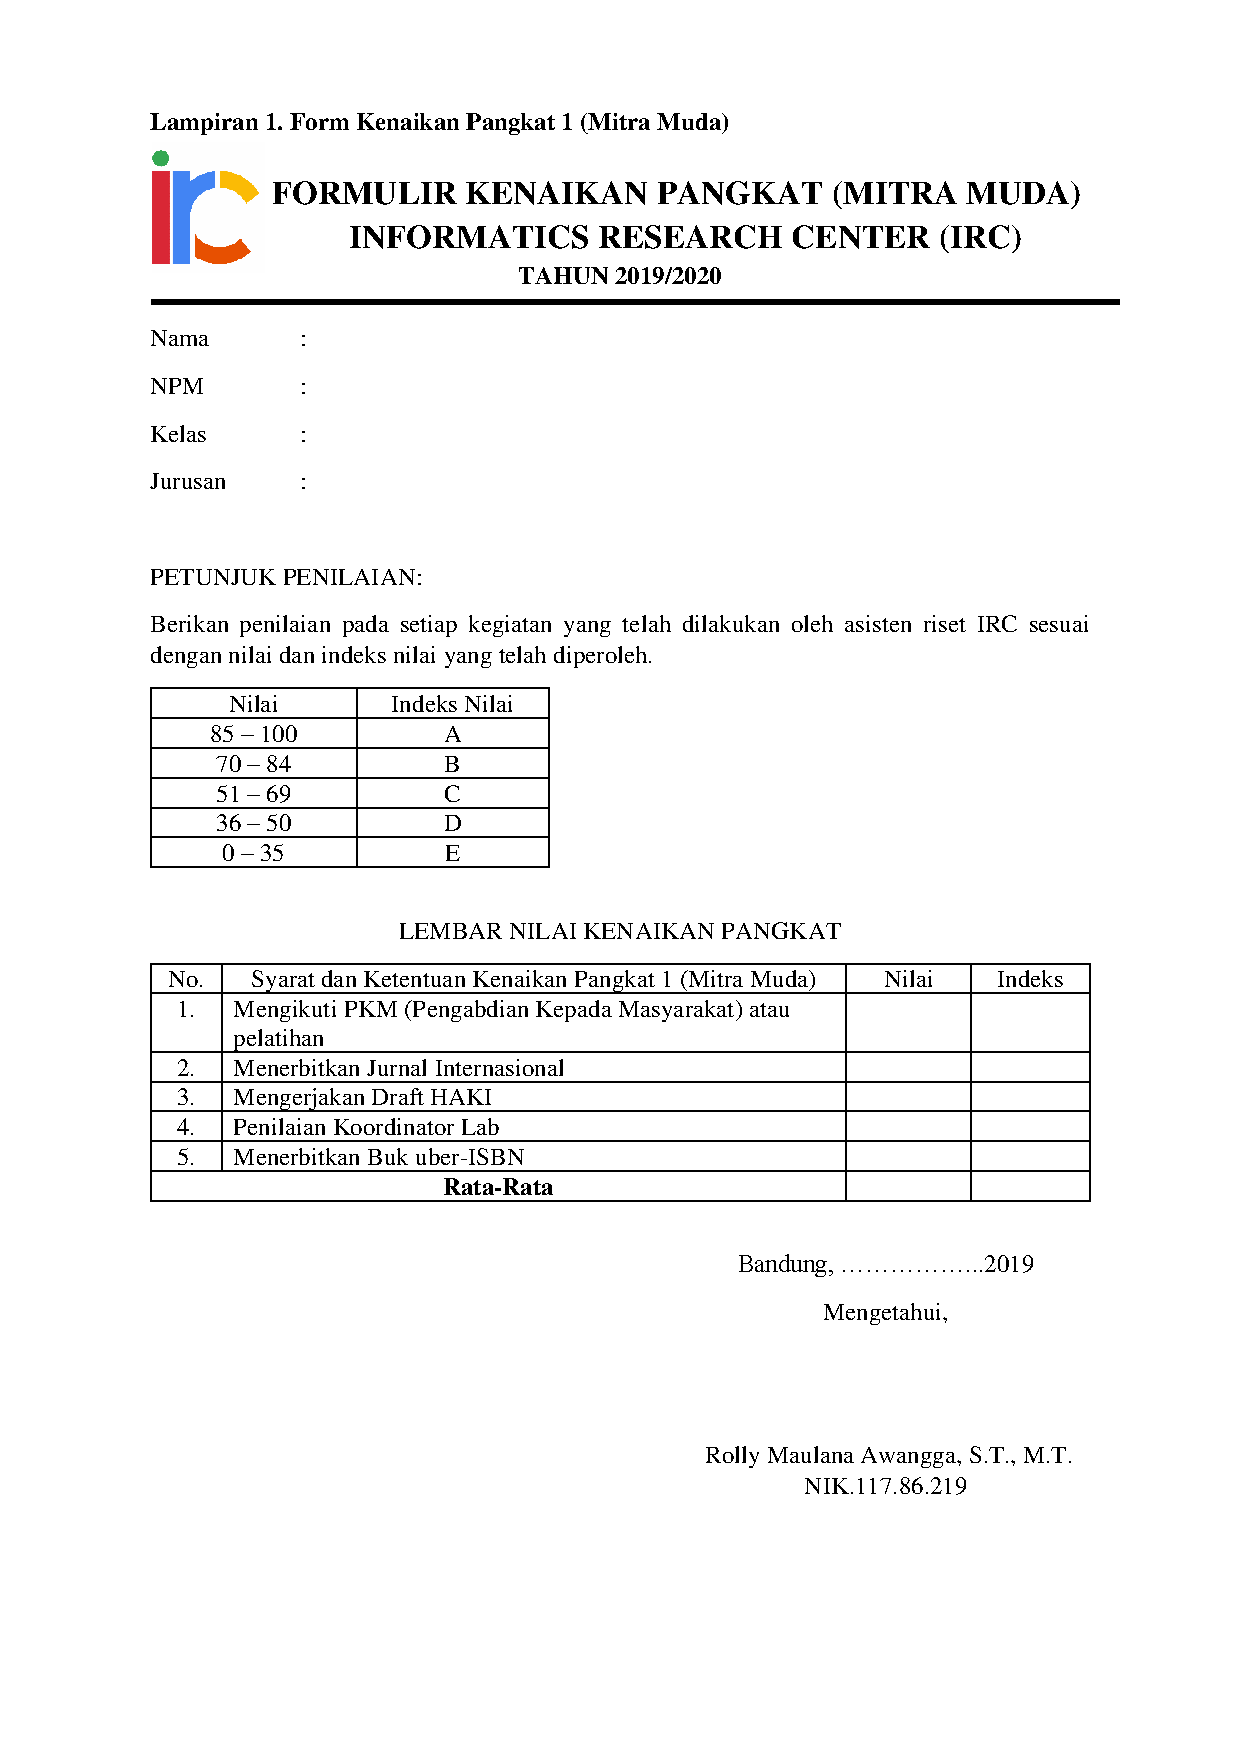
\includepdf[pages={1}]{pangkat1.pdf}      
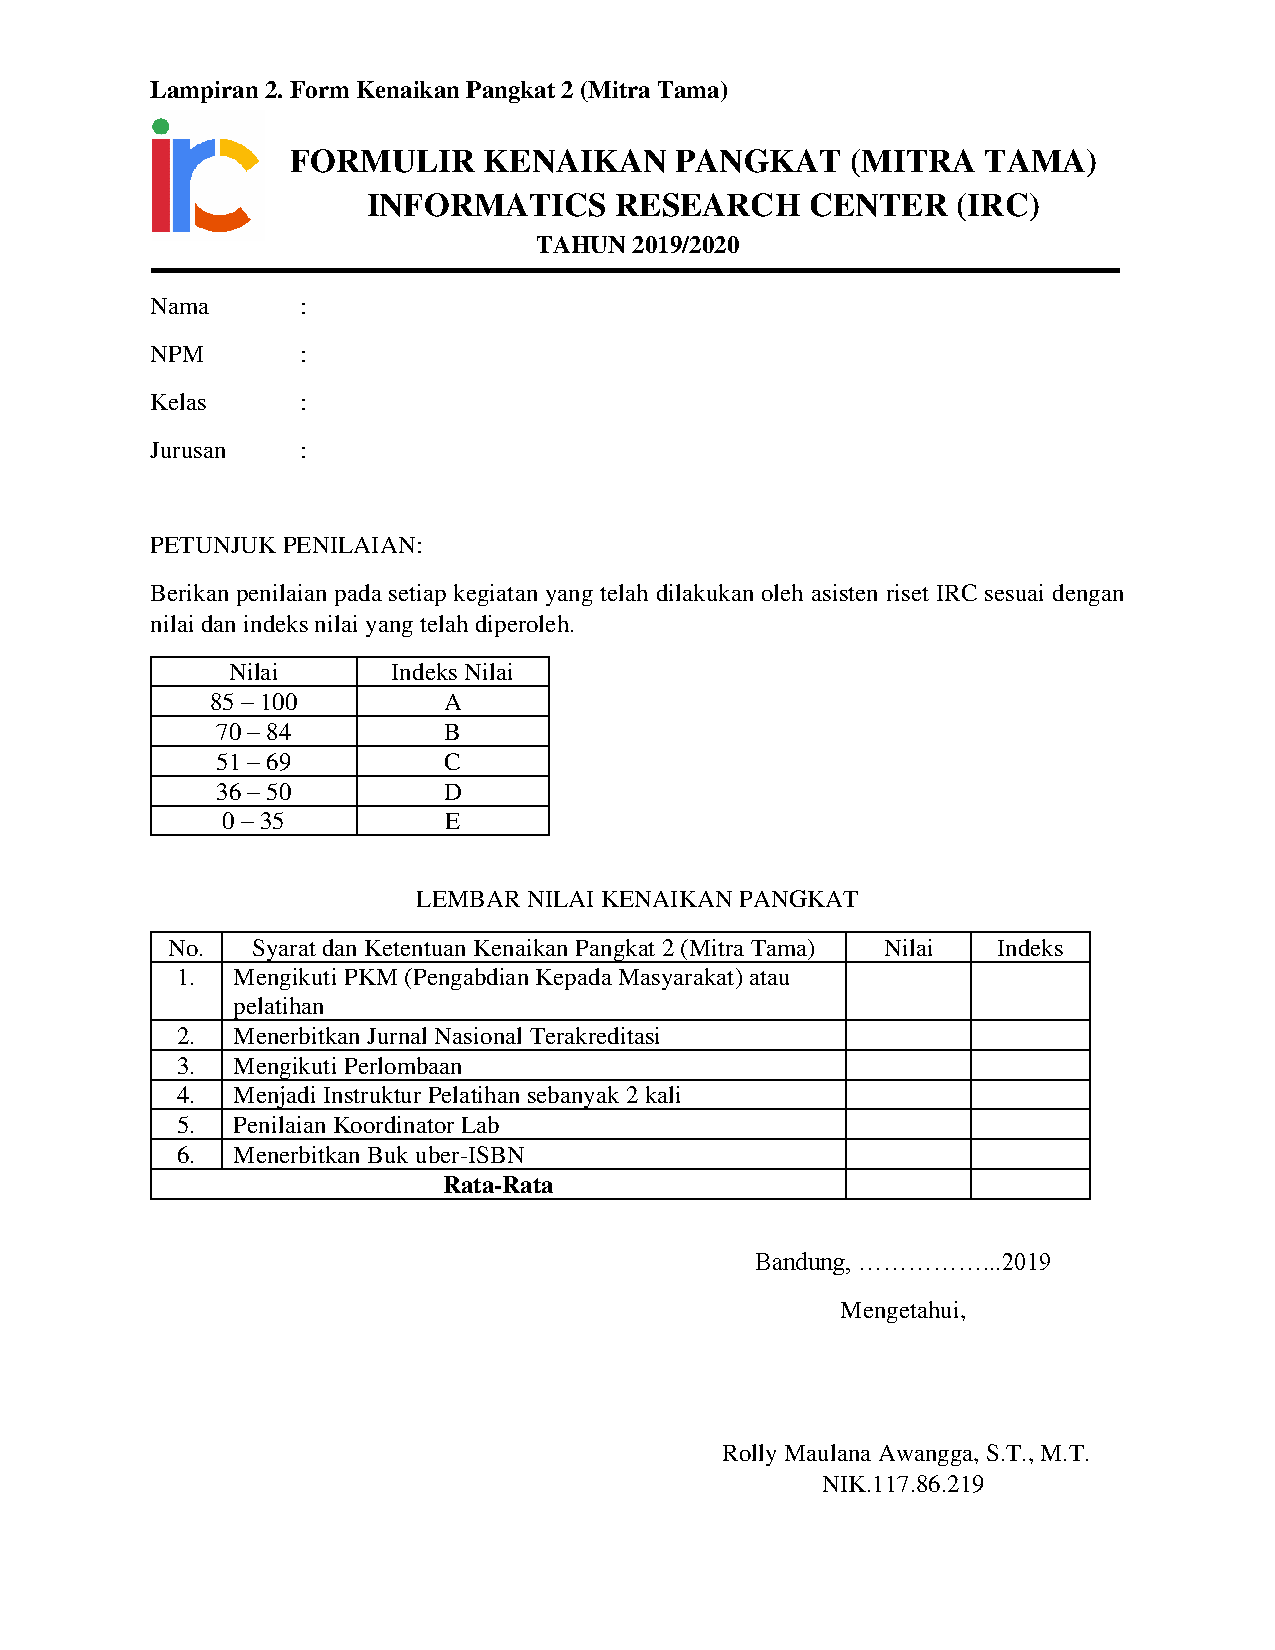
\includepdf[pages={1}]{pangkat2.pdf} 
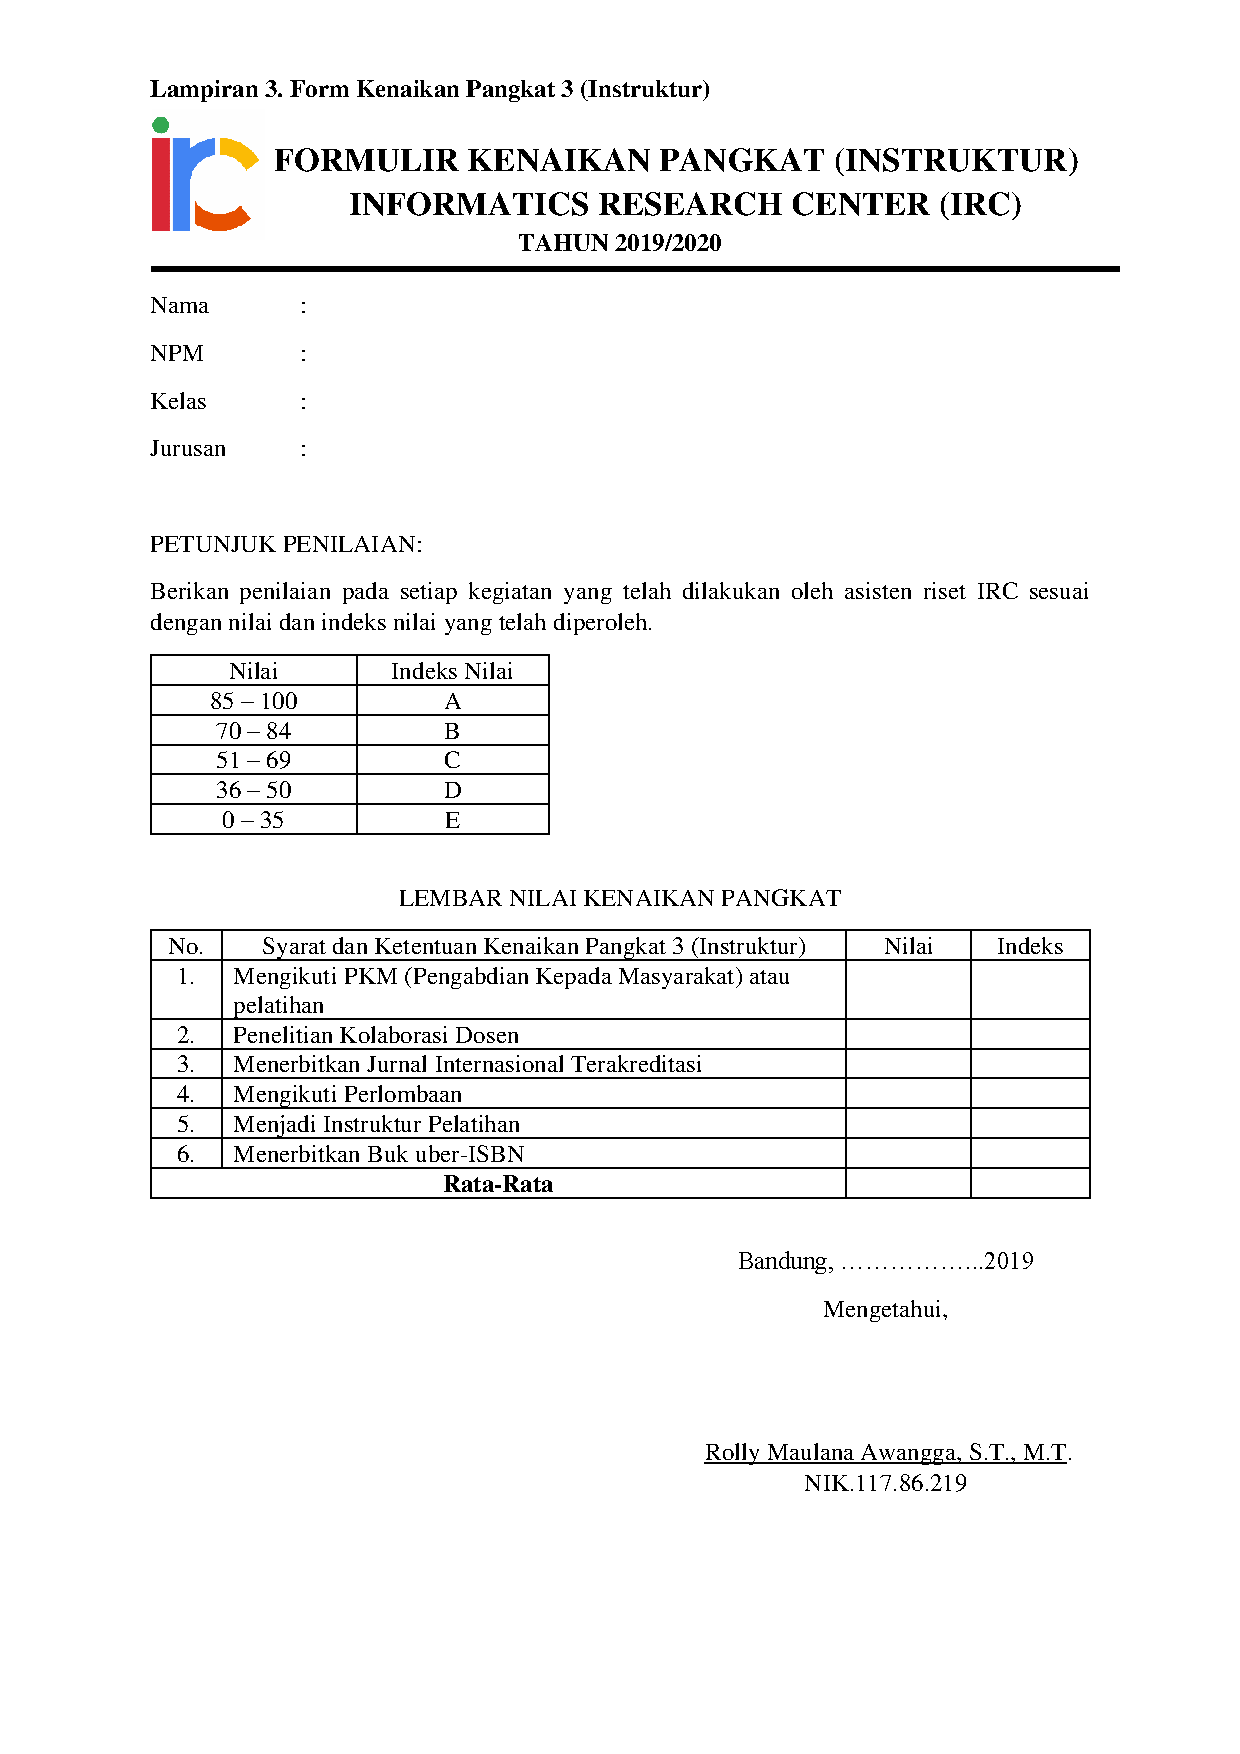
\includepdf[pages={1}]{pangkat3.pdf}

%next line adds the Bibliography to the contents page
\addcontentsline{toc}{chapter}{Bibliography}
%uncomment next line to change bibliography name to references
%\renewcommand{\bibname}{References}
%\bibliography{references}        %use a bibtex bibliography file refs.bib
\bibliographystyle{plain}  %use the plain bibliography style

\end{document}

